% ****** Start of file apssamp.tex ******
%
%   This file is part of the APS files in the REVTeX 4.1 distribution.
%   Version 4.1r of REVTeX, August 2010
%
%   Copyright (c) 2009, 2010 The American Physical Society.
%
%   See the REVTeX 4 README file for restrictions and more information.
%
% TeX'ing this file requires that you have AMS-LaTeX 2.0 installed
% as well as the rest of the prerequisites for REVTeX 4.1
%
% See the REVTeX 4 README file
% It also requires running BibTeX. The commands are as follows:
%
%  1)  latex apssamp.tex
%  2)  bibtex apssamp
%  3)  latex apssamp.tex
%  4)  latex apssamp.tex
%
\documentclass[%
 reprint,
%superscriptaddress,
%groupedaddress,
%unsortedaddress,
%runinaddress,
%frontmatterverbose, 
%preprint,
%showpacs,preprintnumbers,
%nofootinbib,
%nobibnotes,
%bibnotes,
 amsmath,amssymb,
 aps,
%pra,
%prb,
%rmp,
%prstab,
%prstper,
%floatfix,
]{revtex4-1}

\usepackage{graphicx}% Include figure files
\usepackage{dcolumn}% Align table columns on decimal point
\usepackage{bm}% bold math
%\usepackage{hyperref}% add hypertext capabilities
%\usepackage[mathlines]{lineno}% Enable numbering of text and display math
%\linenumbers\relax % Commence numbering lines

%\usepackage[showframe,%Uncomment any one of the following lines to test 
%%scale=0.7, marginratio={1:1, 2:3}, ignoreall,% default settings
%%text={7in,10in},centering,
%%margin=1.5in,
%%total={6.5in,8.75in}, top=1.2in, left=0.9in, includefoot,
%%height=10in,a5paper,hmargin={3cm,0.8in},
%]{geometry}

\usepackage{listings} % used for including computer code 
\usepackage{amsmath}


\begin{document}

\preprint{APS/123-QED}

\title{Observing Doppler's Law by Simulating the Drop of a Whistling Projectile}

\author{Eugene Lytnev}
\affiliation{San Jose State University}
\date{December 11, 2017}

\begin{abstract}
In this project, I tried simulating the Doppler effect for a whistling projectile using two ways to find if I can make the sound effect of a bomb dropping in the movies. The two ways were generating the sound from the Doppler frequency and manipulating the sound directly. I used MoviePy and PyLab for the simulation, and found that one can achieve the appropriate sound effect by placing the observer at the release point of the projectile. I also learned how to use MoviePy as well as some techniques for speeding up Python code.
\end{abstract}

\maketitle

%\tableofcontents

\section{\label{sec:intro}Introduction}

The sound that bombs make as they fall in the World War II movies has fascinated me recently. I wondered how accurate those sounds were to real life and whether that sound actually occurred naturally in the first place. I chose to simulate that sound for this project in Python with Jupyter notebook and MoviePy.

\section{\label{sec:methods}Methods}

I decided to simulate the sound using two methods. The first method would be using the Doppler formula using velocity as an input. The second method would be to interpolate the sound displacing individual audio sample points based on the the time it would take for that sample point to reach the observer.

\subsection{\label{sec:whistle}The Whistle}

To do this, I first needed to figure out what was causing the whistling noise in the first place. To my surprise, the source of the whistle was an actual whistle attached to the tail of the projectile.

I simulated the whistle using a sin function with very diminished harmonics. I used this equation to generate the raw audio for the whistle:

\begin{equation}\label{eq:whistle}
w(t) = \sum_{n=1}^{5} 10^{1-n} \sin{(n f 2 \pi t)}
\end{equation}

Here, $t$ is the time, $f$ is the frequency, and $n$ is the harmonic number.

\subsection{\label{sec:drop}The Drop Simulation}

Next, I needed to get data on the sound source, which was the bomb in this case. I successfully found the aerodynamic data for the Mk-82 Bomb in a paper by the Australian Department of Defense\cite{mk82}. I tried setting up a numeric simulation which would calculate the velocity and position of the fall given initial conditions, but found out to my dismay that, due to the audio needing a very high sample rate, a single pass of this simulation would take more than a day. I did include the code in the appendix on page \pageref{sec:numsim}. Instead, I had to fall back onto a simplified analytic solution to the problem. I ignored drag and used this simple set of kinematics equations to simulate the drop:

\begin{equation}\label{eq:dropx}
x(t) = v_{x0} t + x_0
\end{equation}
\begin{equation}\label{eq:dropy}
y(t) = \frac{1}{2}gt^2+ v_{y0} t + y_0
\end{equation}
\begin{equation}\label{eq:dropvx}
v_x(t) = gt + v_{x0}
\end{equation}
\begin{equation}\label{eq:dropvy}
v_y(t) = gt + v_{y0}
\end{equation}

Here, $x(t)$, $y(t)$, $v_x(t)$, and $v_y(t)$ are the $x$ and $y$ coordinates of the position and velocity, respectively, while $x_0$, $y_0$, $v_{x0}$, and $v_{y0}$ are the respective initial conditions. $t$ is the time and $g$ is the gravitational acceleration constant (I used $g = 9.80$ m/s$^2$).

Using equation \ref{eq:dropy} and the quadratic formula, I also found the final time to be
\begin{equation}\label{eq:droptf}
t_f = \dfrac{-v_{y0} - \sqrt{v_{y0}^2 - 2 g y_0} }{g}
\end{equation}


\subsection{\label{sec:motion}The Motion Relative to the Obsever}

I needed the motion of the projectile relative to the observer. I used the distance formula to get the distance between the projectile and the observer

\begin{equation}\label{eq:dropd}
d(t) = \sqrt{(x(t)-x_{obs})^2 + (y(t)-y_{obs})^2}
\end{equation}
where $x_{obs}$ and $y_{obs}$ are the $x$ and $y$ coordinates of the observer, and $d$ is the distance between the observer and the projectile.

I plugged equations \ref{eq:dropx} and \ref{eq:dropy} into the distance formula and took the derivative to get the velocity of the projectile relative to the observer.

\begin{multline}\label{eq:dropvobs}
v_{obs}(t) = d'(t) = 
\dfrac{v_{x0}(v_{x0}t+x_0-x_{obs})}{d}+\\
\dfrac{(gt+v_{y0})(\frac{1}{2}gt^2+v_{y0}t+y_0-y_{obs})}{d}
\end{multline}

The final code for this simulation can be found on page \pageref{sec:codesim}.

\subsection{\label{sec:timevec}The Time Vector}

At this point, I needed a time vector. I could not simply use \verb|linspace| or \verb|arange| as I needed to make sure that the time aligned nicely with seconds, meaning that every multiple of my sample rate needed to be equal to an integer. To do this, I created the function \verb|timearray| which created a base second and appended it to itself until the needed time has been reached. The final code can be found on page \pageref{sec:codetimearr}.

\subsection{\label{sec:soundspeed}The Average Speed of Sound}

The last thing I needed to define was the average speed of sound between the projectile and the observer. To do this, I used the formula for the speed of sound given temperature, which is 

\begin{equation}\label{eq:rawsspeed}
s = \sqrt{\dfrac{\gamma R}{M} T}
\end{equation}
where $\gamma$ is the adiabatic constant (I used $\gamma = 1.4$ as the constant for air), $R$ is the ideal gas constant (I used $R = 8.314$ J/mol/K), $M$ is the molecular mass of air (I used $M = 0.02897$ kg/mol), and $T$ is the temperature.

Here, I used the standard atmosphere, described in a government report\cite{atmos}, and substituted their equation 7 into their equation 13 to get

\begin{equation}\label{eq:temp}
T(z) = T_0 - \alpha y
\end{equation}
where $T_0$ is the temperature of air at sea level (I used $T_0 = 288.16$ K) and $\alpha$ is a constant equal to $\dfrac{ag}{G}$ from the report\cite{atmos} (This works out to $\alpha = .0065$ K/m).

Substituting equation \ref{eq:temp} into equation \ref{eq:rawsspeed}, I got

\begin{equation}\label{eq:sspeed}
s(y) = \sqrt{\dfrac{\gamma R}{M} (T_0 - \alpha y)}
\end{equation}

I found the average sound speed using the equation

\begin{equation}\label{eq:sspeedint}
\bar{s}  = \dfrac{1}{y_{proj} - y_{obs}}\int^{y_{proj}}_{y_{obs}} s(y) dy
\end{equation}

I created two new constants
\begin{equation}\label{eq:beta}
\beta = \dfrac{2}{3 \alpha}\sqrt{\dfrac{\gamma R}{M}}
\end{equation}

\begin{equation}\label{eq:epsilon}
s_{obs} = \beta (T_0 - \alpha y_{obs})^{\frac{3}{2}}
\end{equation}

Substituting equation \ref{eq:sspeed} into equation \ref{eq:sspeedint} and integrating, I got

\begin{equation}\label{eq:sspeedav}
\bar{s}(y) = \dfrac{\beta(T_0 - \alpha y)^{\frac{3}{2}}-s_{obs}}{y-y_{obs}}
\end{equation}

The final code for this was included in the simulation code on page \pageref{sec:codetimearr}.

\subsection{\label{sec:method1}Method 1: Frequency and the Doppler Equation}

For this method, I just calculated the Doppler shifted frequency at every point in time using the Doppler frequency equation
\begin{equation}\label{eq:doppler}
f'(t) = f \dfrac{s}{s+v_{obs}}
\end{equation}
where $f$ is the emitted frequency.

The final code for this method can be found on page \pageref{sec:codemethod1}.

\subsection{\label{sec:aliasing}Avoiding Aliasing}

Te be certain that the results I was getting were accurate, I decided to cut out samples with frequencies higher than the Nyquist frequency for my audio sample. The Nyquist frequency ($f_N$) is the highest frequency that a data sample can carry without a chance of aliasing, which is when a data sample of a wave has a different frequency to its source wave. We can calculate the Nyquist frequency by dividing the sample rate by two. 

I cut the samples by taking inputting the frequency at each point into this scaled sigmoid function, so that it would fade out the sound instead of just cutting the samples:

\begin{equation}\label{eq:sigma}
\sigma = \dfrac{1}{1+e^{ \frac{5}{30}(f'-f_N)}}
\end{equation}

The final code for this was included in the code for Method 2 on page \pageref{sec:codemethod1}.

\subsection{\label{sec:method2}Method 2: Manual Shifting of Audio Sample}

For this method, I simply took my audio sample and displaced it by the time it took to travel to the observer, which I calculated like so

\begin{equation}\label{eq:sspeedav}
\Delta t = \dfrac{d}{s}
\end{equation}
where, again, d is the distance between the projectile and the observer and s is the average speed of sound. I then subtracted the smallest time value from the entire time array to align the output the two methods.

This resulted in a shifted curve, like in figure \ref{fig:manshift}. All I needed to do then was to interpolate the audio to the original time array, and I had the audio sample I needed.

\begin{figure}\label{fig:manshift}
\centering{
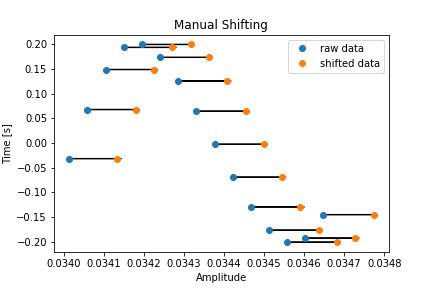
\includegraphics[width=8cm]{manshift.png}
\caption{Manual Shifting of Audio Sample}
}
\end{figure}

The final code for this method can be found on page \pageref{sec:codemethod2}.

\section{\label{sec:results}Results and Discussion}

Using these methods, I was able to create two audio samples which simulated the drop. I added a video graph by plotting the position of the projectile using PyLab and MoviePy. 

I found that the samples were fairly similar. You can see the frequency of the two methods in figure \ref{fig:freqplot}. As you can see there the frequencies align nicely. They do however diverge a bit,  which is definitely a topic that can be explored further.

\begin{figure}\label{fig:freqplot}
\centering{
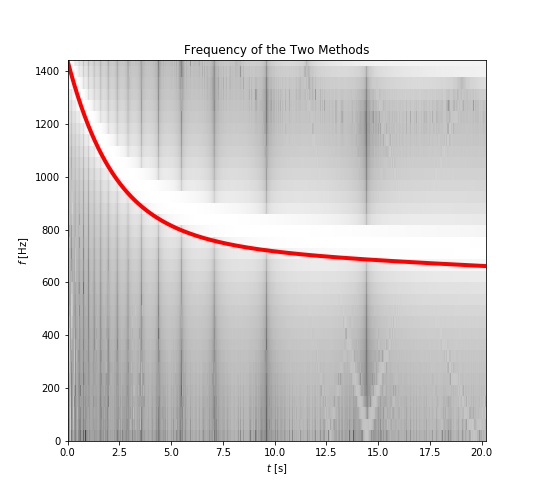
\includegraphics[width=8cm]{freqplot.png}
\caption{Frequency vs time of the audio from Method 1 and Method 2. The spectrograph is from Method 2. It is grey where the frequency is less prominent and white where it is more promnent. The frequency used to generate Method 2 is the red line.}
}
\end{figure}

The resulting video (Fig. \ref{fig:video}), the code, and this report can be found on this project's Github page at \url{https://www.github.com/yogene/p40doppler}.

Interestingly enough, even though I initially thought that it would be impossible to achieve this sound from the ground, given that the projectile is rapidly accelerating towards said ground, I found that if I placed the observer on the ground at the $x$ coordinate of the release point of the projectile, I actually got the typical sound effect.

\begin{figure}\label{fig:video}
\centering{
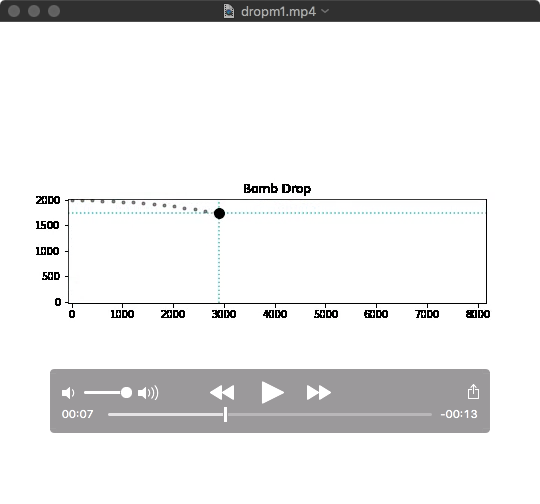
\includegraphics[width=8cm]{video.png}
\caption{The visualization video.}
}
\end{figure}

\section{\label{sec:conclusion}Conclusion}

The diverging frequencies were certainly surprising and it would be interesting to explore why they diverge. Additionally it seems as though it would be possible to significantly speed up the computational solver to a point where it can take a reasonable amount of time. This project helped me learn how to to work with MoviePy and allowed me to dive into techniques for speeding up computations in Python. It also helped me explore some of the math behind the Doppler effect.

%\newpage

\begin{thebibliography}{100}

\bibitem{mk82} Krishnamoorthy, LV, Glass, R, \& Kirk, DR (1997). Measurement of Drag Characteristics of Mk 82 General Purpose Low Drag Bomb using an Aeroballistic Range Facility. DSTO Aeronautical and Maritime Research Laboratory.

\bibitem{atmos} International Civil Aviation Organization, Langley Aeronautical Laboratory. Standard Atmosphere - Tables and Data for Altitudes to 65,800 feet

\end{thebibliography}

\clearpage

\onecolumngrid
\appendix
\section{\label{sec:code}Code}

\subsection{\label{sec:codeinit}Initialization}

\begin{lstlisting}[label=lst:init,language=Python]
from pylab import *
from numba import jit
from moviepy.editor import VideoClip,AudioFileClip,VideoFileClip
from moviepy.audio.AudioClip import AudioArrayClip
from moviepy.video.io.bindings import mplfig_to_npimage
\end{lstlisting}

\subsection{\label{sec:codetimearr}Time Array}

\begin{lstlisting}[label=lst:timearr,language=Python]
def timearray(duration,sampleRate = 44100,overshoot=False):
    '''
    Returns a time array.
    '''
    last_full_second = int(floor(duration))
    partial_seconds = duration % 1.0
    second = linspace(0.,1.,sampleRate+1)[1:]
    time = array([0])
    for i in range(last_full_second): 
        time = concatenate((time,i+second))
    partial_second = last_full_second + second[second <= partial_seconds]
    exact_duration = True if \
        (partial_second[-1] if len(partial_second) > 0 else last_full_second)\
        == duration else False
    if overshoot == True and not exact_duration:
        if len(partial_second) == len(second):
            partial_second = concatenate((partial_second,second[0:1]+last_full_second+1))
        elif len(partial_second) == len(second) - 1:
            partial_second = concatenate((partial_second,second[-1:]+last_full_second))
        else:
            lps = len(partial_second)
            partial_second = concatenate((partial_second,second[lps:lps+1]+last_full_second))
    time = concatenate((time,partial_second))
    return time
\end{lstlisting}

\subsection{\label{sec:coderescale}Audio Rescaling for MoviePy}

\begin{lstlisting}[label=lst:rescale,language=Python]
def rescaleAudio(audio,channels=1):
    '''
    Rescales audio for MoviePy (from -1 to 1)
    '''
    audio = audio - min(audio)
    audio = audio * 2 / max(audio)
    audio = audio - 1
    if shape(audio) == (1):
        audio.reshape((len(audio),1))
        channel = audio[:]
        for i in range(channels-1):
            audio = concatenate((audio,channel),axis=1)
    return audio.reshape((len(audio),1))
\end{lstlisting}

\subsection{\label{sec:codeuservars}User-Set Variables}

\begin{lstlisting}[label=lst:uservars,language=Python]
# initial conditions
pos_x_observer = 0. #m
pos_y_observer = 2000. #m
pos_x_object = 0. #m
pos_y_object = 2000. #m
vel_x_object = 400. #m/s
vel_y_object = 0. #m/s
#m = 250. #kg

# audio settings
whistle_frequency = 1440. #Hz
sample_rate = 44100 #Hz (44100)
\end{lstlisting}

\subsection{\label{sec:codesim}Simulation}

\begin{lstlisting}[label=lst:sim,language=Python]
# sample rate
rate = sample_rate
nyquist = rate/2

# physical constants
g = -9.8 #m/s^2
T0 = 288.16 #K

# mathematical constants
alpha = .0065 # K/m
beta = (2./3.)/alpha*sqrt(1.4*8.314/0.02897)

# variable reassignments
x0 = pos_x_object
v0x = vel_x_object
y0 = pos_y_object
v0y = vel_y_object
xObs = pos_x_observer
yObs = pos_y_observer
x0diff = x0-xObs
y0diff = y0-yObs

# the simulation
drop_time = (-v0y - sqrt(v0y**2 - 2*g*y0))/g
t = timearray(drop_time,rate)
duration = max(t)
one = ones(len(t))
x = v0x*t + x0
y = .5*g*t**2+ v0y*t + y0
vx = g*t + v0x
vy = g*t + v0y
d = sqrt((x-xObs)**2 + (y-yObs)**2)
vObs = (v0x*(v0x*t+x0diff)+(g*t+v0y)*(.5*g*t**2+v0y*t+y0-yObs))/d
sObs = beta*(T0-alpha*yObs)**1.5
s = (beta*(T0-alpha*y)**1.5 - sObs)/(yObs-y)

#print 'Drop time: %.5f s' % drop_time
#print 'Duration: %.5f s' % duration
#print 'Final vel: %.5f m/s' % vObs[-1]
\end{lstlisting}

\subsection{\label{sec:codewhistle}Whistle Function}

\begin{lstlisting}[label=lst:whistle,language=Python]
def whistle(f,t) :
    '''
    Creates a nice sounding whistle given a frequency f and a time array t.
    '''
    summ = 0
    for n in range(1,6): summ += (10**(1-n))*sin(n*f*2*pi*t)
    #summ *= 2**13
    summ /= 5
    return summ
\end{lstlisting}

\subsection{\label{sec:codemethod1}Method 1 Doppler Shift}

\begin{lstlisting}[label=lst:method1,language=Python]
f = whistle_frequency
fdop = (s/(s+vObs))*f
sigma = 1/(1+exp((fdop-(sample_rate/2.))*5/30))
m1aud = whistle(fdop,t)
m1aud *= sigma
m1audio = AudioArrayClip(rescaleAudio(m1aud),rate*2)
m1audio.ipython_display(loop=False,autoplay=False,audio_codec='aac')
\end{lstlisting}

\subsection{\label{sec:codemethod2}Method 2 Doppler Shift}

\begin{lstlisting}[label=lst:method2,language=Python]
rawwhistle = whistle(f,t)
dt = d/s
tdop = t + dt
tdop = tdop - tdop[0]
m2aud = interp(t,tdop,rawwhistle)
m2aud *= sigma
m2audio = AudioArrayClip(rescaleAudio(m2aud),rate*2)
m2audio.ipython_display(loop=False,autoplay=False,audio_codec='aac')
\end{lstlisting}

\subsection{\label{sec:codemoviepy}MoviePy Visualization}

\begin{lstlisting}[label=lst:moviepy,language=Python]
xmin=min(x)-.01*ptp(x)
xmax=max(x)+.01*ptp(x)
xscale=xmax-xmin
ymin=0-.01*y0
ymax=y0+.01*y0
yscale=ymax-ymin
tmin=min(t)-.01*ptp(t)
tmax=max(t)+.01*ptp(t)
tscale=tmax-tmin

fig = plt.figure(figsize=(7.5,7))
ax = fig.add_subplot(111)
skip = int(ceil(len(t)/40))
def make_frame(timestamp):
    i = len(t) - 1 - argmax(t[::-1] <= timestamp)
    ax.clear()
    ax.set_aspect('equal')
    ax.plot([x[i],x[i]],[ymin,ymax],':c',markersize=5)
    ax.plot([xmin,xmax],[y[i],y[i]],':c',markersize=5)
    ax.plot(x[:i+1:skip], y[:i+1:skip],'.k',alpha=.5)
    ax.plot(x[i], y[i],'ok',markersize=10)
    #ax.text(xmin+.01*xscale, ymin+.05*yscale,' t: %.5fsec \n y: %.5fm' % (t[i],y[i]))
    ax.set_xlim(xmin,xmax)
    ax.set_ylim(ymin,ymax)
    #ax.set_xlabel('$x$')
    #ax.set_ylabel('$y$',rotation=0)
    ax.set_title('Bomb Drop')
    return mplfig_to_npimage(fig)

videoclip = VideoClip(make_frame, duration=duration)
audioclip = m1audio
finalclip = videoclip.set_audio(audioclip)
finalclip.ipython_display(fps=30,loop=False,autoplay=False,audio_codec='aac')
finalclip.write_videofile('dropm1.mp4',fps=30,audio_codec='aac')
\end{lstlisting}

\section{\label{sec:numsim}Numeric Simulation}

\begin{lstlisting}[label=lst:numsim,language=Python]
from ipywidgets import FloatProgress, FloatText, IntText
from IPython.display import display
from traitlets import link

rate = 44100
maxtime = 60 #sec

v0 = array([150.,0.]) #m/s
h0 = 2000. #m
x0 = array([0.,h0]) #m
m = 250. #kg
mu = .1
g = -9.8 #m/s^2
area = .27*pi #m^2
ro = 1.225 #kg/m^3

progress = FloatProgress(min=-h0, max=0, description='progress')
height = FloatText(value=0, description='height')
time = FloatText(value=0, description='time')
iteration = IntText(value=0,description='iteration')
#link((progress,'value'),(height,'value'))
display(progress,height,time,iteration)

@jit
def simulate(rate,maxtime,m,mu,area,v0,x0,g,ro):
    second = linspace(0.,1.,rate+1)[1:]
    maxiter = rate * maxtime 
    #maxiter = 10 
    i = 0
    mg = m*g
    t = 0
    v = v0[:]
    lv = sqrt(sum(v**2))
    uv = v/lv
    fg = array([0.,mg])
    fd = uv * .5 * mu * m * lv**2 * area * ro
    f = fg + fd
    a = f / m
    x = x0[:]
    h = x[1]
    F,Fd,Fg = [f],[fd],[fg]
    T,X,V,A = [t],[x],[v],[a]
    #print i,X[i],type(X),type(X[i]),len(X[i]),X[i][1]
    #while X[i][1] > 0 and i < maxiter:
    while h > 0 and i < maxiter:
        last = i
        i += 1
        t = T[i-1] - T[i-1]%1 + second[i%rate]
        dt = t - T[i-1]
        lv = sqrt(sum(v**2))
        uv = v/lv
        fg = array([0.,mg])
        fd = -uv * .5 * mu * m * lv**2 * area * ro
        f = fg + fd
        a = f / m
        v = v + a*dt
        x = x + v*dt
        h = x[1]
        progress.value = -h
        height.value = h
        time.value = t
        iteration.value = i
        F.append(f)
        Fd.append(fd)
        Fg.append(fg)
        T.append(t)
        X.append(x)
        V.append(v)
        A.append(a)
        #print 'i = %d, t = %.5f, h = %.5f' % (i,t,h)
    F,Fd,Fg = array(F),array(Fd),array(Fg)
    T,X,V,A = array(T),array(X),array(V),array(A)    
    return X,V,A,T,F,Fd,Fg
X,V,A,T,F,Fd,Fg = simulate(rate,maxtime,m,mu,area,v0,x0,g,ro)
print m,mu,area,v0,x0,g,ro
t = T
x,y = X.T
\end{lstlisting}



\end{document}
%
% ****** End of file apssamp.tex ******